% % part: 微分方程
% % chapter: 积分方程

% % 有几个前面章节(偏微分方程)的图片要引用


% \documentclass[UTF8]{ctexbook}

% \ctexset{
%     part/number = \chinese{part}
% }
% \usepackage{multirow}
% \usepackage{amsmath}% ams 数学公式
% \usepackage{amsfonts}% ams 数学字体
% \usepackage{bbm}%重影字体
% \usepackage{amssymb,latexsym}% ams 数学符号与LaTeX数学符号
% \usepackage{mathrsfs}% 花式符号
% \usepackage{ntheorem}%定理、定义、证明
%     \theoremstyle{nonumberplain}
%     \theoremheaderfont{\bfseries}
%     \theorembodyfont{\normalfont}
%     \theoremsymbol{$\square$}
%     \newtheorem{Proof}{\hskip 2em 证明}
%     \newtheorem{theorem}{\hspace{2em}定理}[chapter]
%     \newtheorem{definition}{\hspace{2em}定义}[chapter] % 如果没有章, 只有节, 把上面的[chapter]改成[section]
%     \newtheorem{axiom}[definition]{\hspace{2em}公理}
%     \newtheorem{lemma}[definition]{\hspace{2em}引理}
%     \newtheorem{proposition}[definition]{\hspace{2em}命题}
%     \newtheorem{corollary}[definition]{\hspace{2em}推论}
%     \newtheorem{remark}{\hspace{2em}注}[chapter] %类似地定义其他“题头”. 这里“注”的编号与定义、定理等是分开的
%     \newtheorem{Assumption}{\hspace{2em}假设}[chapter]

% %算法伪代码
% %http://blog.csdn.net/lwb102063/article/details/53046265
% \usepackage{algorithm}
% \usepackage{algorithmicx}
% \usepackage{algpseudocode}
%     \floatname{algorithm}{算法}
%     \renewcommand{\algorithmicrequire}{\textbf{输入:}}
%     \renewcommand{\algorithmicensure}{\textbf{输出:}}
% % 罗马数字:示例:\rom{2}
% \makeatletter
% \newcommand*{\rom}[1]{\expandafter\@slowromancap\romannumeral #1@}
% \makeatother

% \usepackage{enumerate}%itemiz环境。\begin{enumerate}[step 1][a)]可以使用 A,a,I,i,1 作为可选项产生 \Alph,\alph,\Roman,\roman,\arabic 的效果
% \usepackage{cite}%参考文献
%     \bibliographystyle{plain}
% \usepackage{extarrows}% 带参数的箭头
% \usepackage{hyperref}% 超链接
% \usepackage{pifont}%然后在正文输入\ding{172}~\ding{211}得到相应数字,要是要①就输入:\ding{172}②就输:\ding{173}
% %\usepackage[CJKbookmarks, colorlinks, bookmarksnumbered=true,pdfstartview=FitH,linkcolor=black,citecolor=black]{hyperref}%超链接的格式设置
% \hypersetup{
%     colorlinks=false,% 去掉超链接颜色
%     pdfborder=0 0 0% 取消超链接的边框
% }
% \usepackage{graphicx}% 图片管理
% \usepackage{caption}
% \usepackage{subcaption}%并排的图各有标题
% \graphicspath{{images/}}% 设置图片搜索路径
% \usepackage{float,varwidth}% 浮动体
% \usepackage{booktabs}% 三线表
% \usepackage{fancyhdr}% 页眉设置
% \usepackage{xcolor}% 颜色宏包
% \usepackage{colortbl}% 彩色表格
% \usepackage{listings}% 代码高亮
% \usepackage{caption}% 对标题进行控制,如让\caption标题的字体缩小一号,同时数字标签使用粗体可以用:\usepackage[font=small,labelfont=bf]{caption}
% \usepackage{xfrac,upgreek}%分别是行间公式如a/b的形式(将原来的命令\frac改成\sfrac)和希腊字体的宏包的
% \usepackage{mathtools}%lgathered和rgathered环境把公式向左向右对齐
% \usepackage{tabularx}%提供自动延伸的表列,(X列格式说明符),文字过长时可以自动转行
% \usepackage{longtable}%长表格
% \usepackage{enumitem}%enumerate宏包的升级
% \usepackage{harpoon}%数学公式的矢量
% \usepackage{bookmark}%目录的书签
% \renewcommand{\headwidth}{\textwidth}%图片并排,这个要列在所有宏包的后面
% \definecolor{codegreen}{rgb}{0,0.6,0}
% \definecolor{codegray}{rgb}{0.5,0.5,0.5}
% \definecolor{codepurple}{rgb}{0.58,0,0.82}
% \definecolor{backcolour}{rgb}{0.95,0.95,0.92}
% \lstset{
%     commentstyle=\color{codegreen},
%     keywordstyle=\color{magenta},
%     numberstyle=\tiny\color{codegray},
%     stringstyle=\color{codepurple},
%     basicstyle=\footnotesize,
%     breakatwhitespace=false,% 断行只在空格处
%     breaklines=true,% 自动断行
%     captionpos=b,% 标题位置
%     keepspaces=true,
%     numbers=left,
%     numbersep=5pt,
%     showspaces=false,
%     showstringspaces=false,
%     showtabs=false,% 显示
%     tabsize=2% TAB 被当作两个空格
% }
% \topmargin=0pt\oddsidemargin=0pt\evensidemargin=0pt
% \textwidth=16.5cm\textheight=23cm\raggedbottom%我这么设置是为了缩小页边距,满足有的文字无法转行
% \pagestyle{headings}%页眉为章节标题,无页脚
% \setlength{\abovecaptionskip}{10pt}
% \setlength{\belowcaptionskip}{-15pt}%图片表格的前后距离设置
% \CTEXsetup[format={\zihao{-3}\raggedright\bfseries}]{section}%设置节的格式


% \begin{document}
% \part{微分方程}
\chapter{积分方程}
\section{积分方程建模}
	\label{sec:积分方程建模}
	\subsection{弦振动积分方程}
		\label{subsec:弦振动积分方程}
		\par
		在偏微分方程建模部分以及引入Sobolev时,我们讨论了弦振动问题的方程,这里,我们再一次来考虑弦振动问题。
		考虑柔软均匀的细弦,将弦两端固定,当受到与平衡位置垂直的外作用力时,弦开始振动。假设运动发生在同一平面(仅上下振动),求不同时间$t$弦上各点的坐标,换句话说,求不同时间$t$的弦曲线。
        \par
        以弦左端点处为坐标原点$O$点,以弦平衡(静止)位置为$x$轴,垂直向上为$u$轴,建立坐标系$xOu$,如图(\ref{fig:弦振动示意图})所示。
        %%%%%%%这个地方有个图片要打
        % \begin{figure}[H]
		% \centering
		% 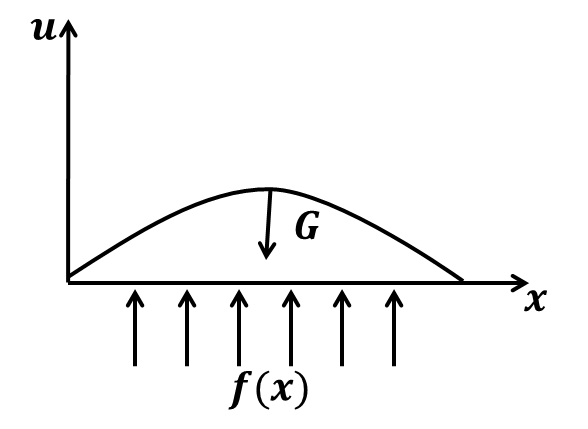
\includegraphics[width=4cm]{images/string_vibration.jpg}
		% \caption{弦振动示意图}
		% \label{fig:弦振动示意图}
		% \end{figure}
        % \textcolor[rgb]{1 0 0}{todo:图片:弦扰动示意图}\\
        设弦长为$l$,外力为$f(x)$,重力为$G$,求$t$时刻各点位置,即$u(x,t)$。
        \par
        先考虑在某一点$x = \xi$处由力$f(x)$所产生的扰动,或者说力$f(x)$使弦在点$x = \xi$处上升了多少,如图(\ref{fig:某点处的弦扰动示意图})所示
        \begin{figure}[H]
		\centering
		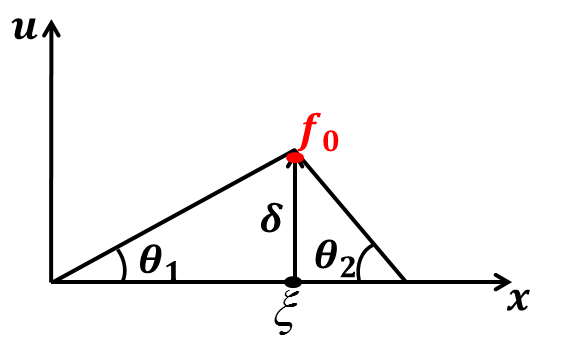
\includegraphics[width=4cm]{images/string_fluctuate_somwhere.jpg}
		\caption{某点处的弦扰动示意图}
		\label{fig:某点处的弦扰动示意图}
		\end{figure}
        % \textcolor[rgb]{1 0 0}{todo:图片:某点处的弦扰动示意图}\\
        设最大上升距离为$\delta$,即扰度(扰动量)。假设扰动量$\delta$是微小的,有
        \begin{align*}
        &\sin \theta_1 \approx \tan \theta _1 = \frac{\delta }{\xi} \\
        &\sin \theta_2 \approx \tan \theta _2 = \frac{\delta }{l - \xi}
        \end{align*}
        设弹性弦张力为$T_0$,在$u$轴方向有受力平衡方程
        \begin{align*}
        	T_0 \sin\theta_1 + T_0\sin\theta_2 = f_0
        \end{align*}
        即
        \begin{align*}
        	T_0\frac{\delta}{\xi} + T_0 \frac{\delta}{l - \xi}  =f_0
        \end{align*}
        所以
        \begin{align*}
        	\delta = \frac{f_0 (l - \xi)}{T_0 l}\xi
        \end{align*}
        在$\xi$处产生的曲线为
        \begin{align*}
	        \phi (x) =
	        \left\{
	        	\begin{aligned}
		        	\frac{f_0 (l - \xi)}{T_0 l} x,\quad 0 \leqslant x \leqslant \xi\\
		        	\frac{f_0 (l - x)}{T_0 l} \xi,\quad \xi \leqslant x \leqslant l
	        	\end{aligned}
	        \right.
        \end{align*}
        \par
        设
        \begin{align*}
	        G(x,\xi) =
	        \left\{
	        	\begin{aligned}
		        	\frac{(l - \xi)}{T_0 l} x,\quad 0 \leqslant x \leqslant \xi\\
			        \frac{(l - x)}{T_0 l} \xi,\quad \xi \leqslant x \leqslant l
	        	\end{aligned}
	        \right.
        \end{align*}
        是单位力$f_0 = 1$所产生的变形曲线,易知$G(x,\xi) = G(\xi,x)$。由于$f(x)$连续,则在微元段$[\xi,\xi+\mathrm{d} \xi]$上的作用力为
        \begin{align*}
        	f_0 = f(\xi) \mathrm{d} \xi
        \end{align*}
        所以微元上的扰动曲线为
        \begin{align*}
        	G(x,\xi) f(\xi)\mathrm{d} \xi
        \end{align*}
        所以整体的扰动曲线(弦曲线)为微元累加
        \begin{align}
        	\label{弦振动积分方程}
        	u(x) = \int_0^l G(x,\xi) f(\xi)\mathrm{d} \xi
        \end{align}

	\subsection{人口增长积分方程}
		\label{subsec:人口增长积分方程}
		我们在常微分方程建模部分讨论了人口增长模型,下面再简单讨论一下人口增长模型。设$t_0$时刻的人口总数为$n_0$,设$f(t,\tau)$表示$\tau$时刻出生的到$t$时刻仍然存活的人占$\tau$时刻出生人数的比例,设$r(t)$为出生率,则$t$时刻人口总数为
		\begin{align*}
			n(t) = n_0 + \int_{t_0}^tf(t,\tau) r(\tau)\mathrm{d} \tau
		\end{align*}
		假设出生率$r(t)$仅与$t$时刻的人口总数成正比,即
		\begin{align*}
			r(t) = k n(t)
		\end{align*}
		则有
		\begin{align}
			\label{人口增长积分方程}
			n(t) - k\int_{t_0}^tf(t,\tau) n(\tau)\mathrm{d} \tau = n_0
		\end{align}
		当$f(t,\tau)$确定之后,即可得到$n(t)$。

\section{积分方程基本内容}
	\label{sec:积分方程基本内容}
	上面介绍的弦振动方程(\ref{弦振动积分方程})和人口增长方程(\ref{人口增长积分方程})就是积分方程模型。积分方程与常微分方程相似,微分方程是$y$与其微分$y'$的方程,积分方程是$y$与其积分$\int f$的方程。积分方程的起源很早,早在1782年,Laplace就运用积分变换
	\begin{align*}
		\phi (x) = \int_0^\infty e^{-xy} \phi(y) \mathrm{d}y
	\end{align*}
	来求解微分方程。
	1826年,Poisson在研究磁场理论时获得了一类积分方程
	\begin{align*}
		\phi (x) = f(x) + \lambda \int_0^x k(x- s) \mathrm{d}s
	\end{align*}
	其中:$\phi(x)$为未知函数,$f,k$为已知函数,$\lambda$为参数。1889年,duBois-Raynod首次提出“积分方程”的名称。1909年,瑞典数学家Erik Ivar Fredholm首次解决了Fredholm方程
	\begin{align*}
		\phi (x) = f(x) + \int_a^b k(x- s) \mathrm{d}s
	\end{align*}
	\par
	通常,将积分号下有未知函数$\phi(x)$的方程为积分方程。就一维情况来看,积分方程的任务仍然是求函数$\phi(x)$使其满足一定的条件(积分方程),积分方程的概念可以由一维推广到高维。下面,我们仅就一维积分方程进行介绍。
	积分方程的一般形式为
	\begin{align*}
		A(x)\phi(x) = \lambda \int_{a(x)}^{b(x)} k(x,s) F[\phi(s)]\mathrm{d}s + f(x) \quad a(x) \leqslant x \leqslant b(x)
	\end{align*}
	其中:$A,k,f$为已知函数,$a(x),b(x)$为已知函数(可以为常数),$\phi(x)$为待求函数,$F[\phi(x)]$为$\phi(x)$的已知泛函,$k(x,s)$核为积分方程的核,$f(x)$称为自由项,$\lambda$为参数。
	\paragraph{Fredholm方程和Volterra方程}
	若泛函$F[\phi(x)]$为$\phi(x)$的线性泛函,则称积分方程为线性积分方程,否则为非线性积分方程。对一般的线性积分方程
	\begin{align*}
		A(x)\phi(x) = \lambda \int_{a(x)}^{b(x)} k(x,s) \phi(s)\mathrm{d}s + f(x)
	\end{align*}
	若积分限$a(x),b(x)$为常数$a,b$,则称为Fredholm方程。若积分限中有一个非常数,如$a(x)$或者都为函数,则称为Volterra方程。后面,我们主要讨论这两种方程的解法。
	\paragraph{第一类方程和第二类方程}
	第一类积分方程的未知函数仅出现在积分号内。第一类Fredholm积分方程为
	\begin{align*}
		\lambda \int_{a}^{b} k(x,s) \phi(s)\mathrm{d}s + f(x) = 0
	\end{align*}
	第一类Volterra积分方程为
	\begin{align*}
		\lambda \int_{a}^{x} k(x,s) \phi(s)\mathrm{d}s + f(x) = 0
	\end{align*}
	第二类积分方程的未知函数即在积分号内,也在积分号外。第二类Fredholm积分方程为
	\begin{align*}
		\phi(x) = \lambda \int_{a}^{b} k(x,s) \phi(s)\mathrm{d}s + f(x)
	\end{align*}
	第二类Volterra积分方程为
	\begin{align*}
		\phi(x) = \lambda \int_{a}^{x} k(x,s) \phi(s)\mathrm{d}s + f(x)
	\end{align*}
	\paragraph{方程的分类}积分方程按核的性质可以分为:核积分方程、弱奇性核积分方程和奇异积分方程。
	\par
	1.当$k(x,s)$是二元连续函数或者平方可积函数时,称$k(x,s)$为核,积分方程为核积分方程。
	\par
	2.当$k(x,s) = \frac{k_0(x,s)}{(x-s)^\alpha}(0<\alpha<1)$时,$k_0(x,s)$为有界函数,则称积分方程为弱奇性核积分方程。
	\par
	3.当$k(x,s) = \frac{a(x,t)}{x-t}$,其中:$a(x,t)$关于$x,t$的偏导数存在。当$\alpha = 1$时,
	\begin{align*}
		\int_a^b k(x,s) \phi(s) \mathrm{d}s = \int_a^b\frac{a(x,s)}{x-s}\phi(x) \mathrm{d}s
	\end{align*}
	在通常意义下是发散的,但是如果对$\phi(x)$加上一定的限制,使
	\begin{align*}
		\lim_{\varepsilon \rightarrow 0} \int_a^{x - \varepsilon} k(x,s) \phi(s) \mathrm{d}s + \int_{x+\varepsilon}^b k(x,s) \phi(s) \mathrm{d}s
	\end{align*}
	存在,即在Cauchy主值积分意义下存在,则称$k(x,s)$为Cauchy奇性核。当$\alpha>1$时,即使在Cauchy主值积分意义下
	\begin{align*}
	\int_a^b k(x,s)\phi(s) \mathrm{d}s
	\end{align*}
	也不存在,则称核为超奇性核,积分方程为超奇性积分方程。
	\par
	如果$k(x,s) = k(s,x)$,则称$k(x,s)$为对称积分核;如果$k(x,s) = k(l-s)$,则称$k(x,s)$为卷积核。如果积分方程中的$f(x) = 0$,则称积分方程为齐次积分方程。
	\paragraph{微分积分方程}如果在积分方程中加入微分项,或者在微分方程中加入积分项,则可以形成如下形式的微分积分方程
	\begin{align*}
		y^{(n)}(x) = C_n + \int_0^x F(x,y(x),y'(x),\dots,y^{(n)}(x))\mathrm{d}x
	\end{align*}

\section{积分方程解的存在唯一性}
	\label{sec:积分方程解的存在唯一性}
	\subsection{Fridholm定理}
		\par
		考虑如下Fredholm积分方程
		\begin{align}
			\label{F积分方程}
			\phi(x) - \lambda\int_a^bk(x,s)\phi(s)\mathrm{d}s = f(x)
		\end{align}
		其中:$f(x) \in L^2(\Omega)$,$k(x,y)\in L^2(\Omega)$。
        \begin{definition}[伴随齐次方程]
        我们称
        \begin{align}
            \label{伴随齐次方程}
            \phi(x) - \lambda\int_a^bk(x,s)\phi(s)\mathrm{d}s = 0
        \end{align}
        为积分方程(\ref{F积分方程})的伴随齐次方程。任给$\lambda$,它显然有平凡解$\phi(x) \approx 0$,但当$\lambda$取某些值时,它可能有不恒等于$0$的非平凡解。
        \end{definition}
        \begin{definition}[特征值]
        使伴随齐次方程(\ref{伴随齐次方程})有非平凡解的$\lambda$值为方程的特征值,对应的非平凡解称为方程(\ref{伴随齐次方程})的特征函数。
        \end{definition}
        \begin{definition}[共轭方程]
        我们称
        \begin{align*}
            \phi(x) = \lambda\int_a^b \overline{k(s,x)}\phi(s)\mathrm{d}s + f(x)
        \end{align*}
        为积分方程(\ref{F积分方程})的共轭方程。$\overline{k(s,x)}$为核$k(x,s)$的共轭核,即把原来的$k(x,s)$中的自变量呼唤,再取复共轭所得的核。
        \end{definition}
        \begin{theorem}[Fridholm定理]
        Fridholm定理即为Fridholm积分方程(\ref{F积分方程})的解存在唯一定理。对方程(\ref{F积分方程})
        \begin{align*}
            \phi(x) - \lambda\int_a^bk(x,s)\phi(s)\mathrm{d}s = f(x)
        \end{align*}
        \ding{172}当且仅当其对应的伴随齐次方程仅有零解时,原方程对任意$f(x)\in L^2(\Omega)$在$L^2$内有唯一解。\\
        \ding{173}若对应的伴随齐次方程有非零解时,则当且仅当$f(x)$与伴随齐次共轭方程
        \begin{align*}
            \phi(x) - \lambda\int_a^b \overline{k(s,x)}\phi(s)\mathrm{d}s = 0
        \end{align*}
        的一切解$\phi(x)$正交时,原方程在$L^2$内有解(不唯一)。\\
        \ding{174}原方程与伴随齐次共轭方程的解空间都是有限维的,而且维数相同。\\
        \ding{175}在平面上任何有界区域内,原方程至多包含有限个特征值。
        \end{theorem}

\section{积分方程数值解法}
	% \label{sec:积分方程数值解法}
	积分方程的求解本质仍然是求$f(x)$。在积分方程部分,我们将$f(x)$记为$\phi(x)$,且论域为$L^2(I)$,$I = [a,b]\in R$。我们仿照微分方程中的有限元法和谱方法来研究一下积分方程。
	\subsection{第二类Fredholm积分方程的数值方法}
		\label{subsec:第二类Fredholm积分方程的数值方法}
		设$\{\varphi_i(x)\}_{i =1}^n$是$L^2(I)$中的完备函数系,可以是正交的,我们可以将待求函数$\phi(x)$用$\{\varphi_i(x)\}$展开,由于基组里$n\rightarrow \infty$,不妨设定为有限项$n$
		\begin{align*}
			\phi(x) \approx \sum_{i =1}^n c_i \varphi_i(x)
		\end{align*}
		\par
		这样,原问题求$\varphi(x)$就变为在给定基组$\{\varphi_i(x)\}_{i =1}^n$之后,求系数$\{c_i\}_{i =1}^n$。将展开后的$\varphi(x)$带回第二类Fredholm积分方程中
		\begin{align}
			\label{第二类Fredholm积分方程}
			\phi(x) = \lambda \int_{a}^{b} k(x,s) \phi(s)\mathrm{d}s + f(x)
		\end{align}
		有
		\begin{align*}
			\sum_{i =1}^n c_i \varphi_i(x) \approx \lambda \sum_{i =1}^n c_i \int_{a}^{b} k(x,s) \varphi_i(s)\mathrm{d}s + f(x)
		\end{align*}
		\par
		我们令
		\begin{align*}
			R(x) = \sum_{i =1}^n c_i \varphi_i(x) - \lambda \sum_{i =1}^n c_i \int_{a}^{b} k(x,s) \varphi_i(s)\mathrm{d}s - f(x)
		\end{align*}
		为残差。

		\subsubsection{配置法}
			\label{subsubsec:配置法}
			\par
			如果我们要求$R(x)$在$[a,b]$的$n$个离散点$\{x_i\}_{i = 1}^n$处的函数值为$0$,则可以得到$n$个方程组,$n$个参数$\{c_i\}_{i = 1}^n$可解。
			\begin{align}
				\label{配置法的方程组}
				\sum_{i =1}^n c_i \varphi_i(x_k) - \lambda \sum_{i =1}^n c_i \int_{a}^{b} k(x_k,s) \varphi_i(s)\mathrm{d}s = f(x_k)  \quad k = 1,2,\dots,n
			\end{align}
			注:上面我们将$[a,b]$离散划分为$n$段,且有$n$个基函数$\varphi_i$。当然基函数的个数可以不取$n$,为了方便,也为了后面分段多项式的运用,我们令离散化段数和基函数个数相等,为$n$。
			\par
			将上述方程组(\ref{配置法的方程组})表示成矩阵的形式,有
			\begin{align}
				\label{配置法方程组的矩阵形式}
				\begin{pmatrix}
				\varphi_{11} - \lambda k_{11}& \varphi_{21} - \lambda k_{21} &\dots &\varphi_{n1} - \lambda k_{n1}\\
				\varphi_{12} - \lambda k_{12}& \varphi_{21} - \lambda k_{22} &\dots &\varphi_{n2} - \lambda k_{n2}\\
				\vdots & \vdots & \ddots& \vdots \\
				\varphi_{1n} - \lambda k_{1n}& \varphi_{2n} - \lambda k_{2n} &\dots &\varphi_{nn} - \lambda k_{nn}
				\end{pmatrix}
				\begin{pmatrix}
				c_1 \\
				c_2 \\
				\vdots\\
				c_n \\
				\end{pmatrix}
				=
				\begin{pmatrix}
				f_1 \\
				f_2 \\
				\vdots\\
				f_n \\
				\end{pmatrix}
			\end{align}
			其中:$\varphi_{ik} = \varphi_i(x_k)$,$k_{ik} = \int_a^b k(x_k,s)\varphi_i(s)\mathrm{d}s$,$f_k = f(x_k)$,$k = 1,2,\dots,n$
			\par
			上面这种要求残差$R(x)$在离散点$\{x_i\}_{i = 1}^n$的取值为$0$的方法称为配置法,或者是配点法。

		\subsubsection{Galerkin法}
			\label{subsubsec:Galerkin法}
			\par
			设$\{\varphi_i\}_{i = 1}^n$是$L^2(I)$的带权$\rho(x)$的正交基(例如前面介绍的Chebyshev多项式和Jacobi多项式等)
			\begin{align*}
				\int_a^b \rho(x) \varphi_i(x) \varphi_j(x) \mathrm{d}x = C_i \delta_{ij}
			\end{align*}
			Galerkin方法要求残差$R(x)$与$\rho(x)\varphi_i(x)$的内积为$0$,注意是$\forall \varphi_i(x) \in \varPhi$,即
			\begin{align*}
				\int_a^b \rho (x) R(x) \varphi_i(x)\mathrm{d}x = 0 \quad i = 1,2,\dots,n
			\end{align*}
			由此,仍可以得到$n$个线性方程组(\ref{配置法方程组的矩阵形式}),但矩阵中的元素计算方法变为如下方式
			\begin{align*}
				&\varphi_{ik} = \int_a^b\rho (x)\varphi_i(x) \varphi_k(x) \mathrm{d}x \\
				&k_{ik} = \int_a^b \left[\int_a^b k(x,s)\varphi_i(s)\mathrm{d}s\right] \rho (x) \varphi_k(x) \mathrm{d}x\\
				&f_k = \int_a^b f(x) \rho(x) \varphi_k(x)\mathrm{d}x
			\end{align*}

		\subsubsection{矩量法}
			\label{subsubsec:矩量法}
			\par
			矩量法要求残差$R(x)$关于原点的$k$阶矩为$0$,即$\forall k \in [1,2,\dots,n]$,有
			\begin{align*}
				\int_a^bR(x) x^k \mathrm{d}x
			\end{align*}
			由此,亦可以得到$n$个线性方程(\ref{配置法方程组的矩阵形式}),这个方程组的矩阵中的元素计算方法变为如下方式
			\begin{align*}
				&\varphi_{ik} = \int_a^b\varphi_i(x) x^k \mathrm{d}x \\
				&k_{ik} = \int_a^b \left[ \int_a^b k(x,s)\varphi_i(s)\mathrm{d}s \right] x^k \mathrm{d}x\\
				&f_k = \int_a^b f(x)x^k\mathrm{d}x
			\end{align*}

		\subsubsection{数值求积公式法}
			\label{subsubsec:数值求积公式法}
			对第二类Fredholm积分方程(\ref{第二类Fredholm积分方程}),设
			\begin{align}
				\label{数值积分公式}
				\int_a^b f(x) \mathrm{d}x \approx \sum_{j = 1}^n A_j f(x_j)
			\end{align}
			为数值积分公式。其中:$x_j\in [a,b]$为区间离散点,$A_j$为求积系数。不妨对积分方程(\ref{第二类Fredholm积分方程})运用数值积分公式,有
			\begin{align*}
				\phi(x) \approx \lambda \sum_{j = 1}^n k(x,x_j) \phi(x_j) + f(x)
			\end{align*}
			\par
			这就像我们在前面弦振动里面分析的那样,某一点的坐标值$\varphi(x)$是所有点累加起来形成的,当计算$x = x_i$点的函数值$\varphi(x_i)$时,有
			\begin{align*}
				\phi(x_i) \approx \lambda \sum_{j = 1}^n k(x_i,x_j) \phi(x_j) + f(x_i)
			\end{align*}
			在$[a,b]$内取$n$个离散点$\{x_i\}(i = 1,2,\dots,n)$,会有$n$个方程,求之,即可得到$\phi(x_i)$。不妨令$\phi_i = \phi(x_i),k(x_i,x_j) = k_{ij},f_i = f(x_i)$,于是有
			\begin{align*}
				\phi_i \approx \lambda \sum_{j = 1}^n k_{ij} \phi_j + f_i \quad i = 1,2,\dots,n
			\end{align*}
			上面共有$n$个参数$\{\phi_i\}$,共有$n$个方程,所以可解。
			\par
			上面遗留的问题是:对数值积分公式(\ref{数值积分公式}),如何确定公式中的$x_j$和$A_j$?总得来说,我们该如何确定数值积分公式?\\
			\textbf{矩形法}
			\begin{align*}
				&x_k = a+(k - 1) \frac{(b-a)}{n} \quad k = 1,2,\dots,n\\
				&A_k = \frac{b-a}{n}
			\end{align*}
			\textbf{梯形法}
			\begin{align*}
				&x_k = a+(k - 1) \frac{(b-a)}{n} \quad k = 1,2,\dots,n\\
				&A_1 = A_n \frac 12\frac{b-a}{n - 1}\\
				&A_k = \frac{b-a}{n - 1} \quad k = 1,2,\dots,n-1
			\end{align*}
			\textbf{Simpson公式}
			\begin{align*}
				&x_{2k+1} = a+2k \frac{(b-a)}{2n} \quad k = 0,1,\dots,n\\
				&A_1 = A_{2n+1} \frac 13\frac{b-a}{2n}\\
				&A_{2k} = \frac{4}{3} \frac{b-a}{2n} k = 1,2,\dots,n\\
				&A_{2K+1} = \frac{2}{3} \frac{b-a}{2n}  \quad k = 1,2,\dots,n-1
			\end{align*}
		\subsubsection{数值求积公式结合谱方法}
			\label{subsubsec:数值求积公式结合谱方法}
			\par
			如果对积分方程同时使用数值积分公式和谱方法,则会有下面的一系列数值积分-多项式方法。在对积分方程(\ref{第二类Fredholm积分方程})中的积分项使用数值积分公式(\ref{数值积分公式})之前(或者之后),将待求函数$\phi(x)$用谱分析的正交多项式表示则可得到数值求积公式结合谱方法。\\
			\textbf{Gauss-Legendre公式}
			\par
			求如下积分
			\begin{align*}
				\int_{-1}^1 f(x) \mathrm{d}x = \sum_{k = 1}^n A_k f(x_k)
			\end{align*}
			高斯点$x_k$满足以下要求
			\begin{align*}
				&P_n(x_k) = 0 \quad k = 1,2,\dots,n\\
				&A_k = \frac{2(1-x_k^2)}{[nP_{n-1}(x_k)]^2}\quad k = 1,2,\dots,n
			\end{align*}
			其中:$P_n(x)$是$n$阶Legendre多项式(\ref{eq:Legendre函数的一般形式})。\\
			\textbf{Gauss-Laguerre公式}
			\par
			求如下积分
			\begin{align*}
				\int_{0}^{-\infty} e^{-x}f(x) \mathrm{d}x = \sum_{k = 1}^n A_k f(x_k)
			\end{align*}
			高斯点$x_k$满足以下要求
			\begin{align*}
				&L_n(x_k) = 0 \quad k = 1,2,\dots,n\\
				&A_k = \frac{(n!)^2}{x_k[L_n'(x_k)]^2}\quad k = 1,2,\dots,n
			\end{align*}
			其中:$L_n(x)$是$n$阶Laguerre多项式(\ref{eq:Laguerre多项式一般形式})。\\
			\textbf{Gauss-Hermitte公式}
			\par
			求如下积分
			\begin{align*}
				\int_{-\infty}^{\infty} e^{-x^2}f(x) \mathrm{d}x = \sum_{k = 1}^n A_k f(x_k)
			\end{align*}
			高斯点$x_k$满足以下要求
			\begin{align*}
				&H_n(x_k) = 0 \quad k = 1,2,\dots,n\\
				&A_k = \frac{2^{n+1}n!\sqrt{\pi}}{[H_n'(x_k)]^2}\quad k = 1,2,\dots,n
			\end{align*}
			其中:$H_n(x)$是$n$阶Hermitte多项式(\ref{eq:Hermite多项式一般形式})。\\
			\textbf{Gauss-Lobatto公式}
			\par
			求如下积分
			\begin{align*}
				\int_{-1}^{1} f(x) \mathrm{d}x = \frac{2}{n(n+1)} [f(-1) + f(1)] + \sum_{k = 2}^{n-1} A_k f(x_k)+R_n(f)
			\end{align*}
			高斯点$x_k$满足以下要求
			\begin{align*}
				&P_n'(x_k) = 0 \quad k = 1,2,\dots,n\\
				&A_k = \frac{2}{n(n+1)[P_n(x_k)]^2} \quad k = 1,2,\dots,n
			\end{align*}
			其中:$P_n(x)$是$n$阶Legendre多项式。
			\par
			对于被积区间为$[a,b]$,令方程(\ref{第二类Fredholm积分方程})中的$s$为
			\begin{align*}
				s = \frac{1}{2} [(b-a)t +(b+a)]
			\end{align*}
			可以将$s$在$[a,b]$上的积分映射到$t$在$[-1,1]$上的积分,然后再用上面的积分公式对变量$t$进行求解即可。

	\subsection{第二类Volterra积分方程的数值方法}
		\label{subsec:第二类volterra积分方程的数值方法}
		\par
		考虑如下形式的第二类volterra积分方程
		\begin{align}
			\label{第二类volterra积分方程}
			\phi(x) = \int_{a}^{x} k(x,s) \phi(s)\mathrm{d}s + f(x) \quad a \leqslant s \leqslant x \leqslant b
		\end{align}
		仍然假设$[a,x]$上的数值积分公式为
		\begin{align*}
			 \int_a^x f(x) \mathrm{d}x \approx \sum_{k = 1}^n A_k f(x_k)
		\end{align*}
		对第二类volterra积分方程(\ref{第二类volterra积分方程})使用数值积分公式,有
		\begin{align*}
			\phi(x) \approx \sum_{k = 1}^n A_k k(x,x_k) \phi(x_k) + f(x) \quad a \leqslant x_k \leqslant x \leqslant b
		\end{align*}
		其中:$n$为区间$[a,x]$的离散点数。对每一个点$x_i$,其函数值$\phi(x_i)$都是其$[a,x_i]$的累加。
		\par
		我们可以选用不同的数值积分公式,得到不同的结果。进一步,如果对积分方程中的待求函数$\phi(x)$用谱方法中的正交多项式替代,则可得到数值积分结合谱方法。




% \end{document}
